\subsection{Pictogram}
\label{sub:pictogram}
%Intro
%What is a pictogram?
In the context of this report a pictogram is defined thus:
\emph{A pictogram is an image representing a living being, a physical object or some form of action.}
Pictograms can contain a text-label, describing the respective images, for clarification. There is currently no standard for the layout or contents of pictograms, due to the specific needs and opinions of the users. User \textbf{A} might like to have black and white images with text labels whereas user \textbf{B} might want colorful images without text. The images can themselves vary from cartoons to photographic representations.
Pictograms are commonly used as means of communication, especially by those requiring assistance with communicating, including but not limited to individuals with autism.

\subsubsection*{Current Use}
\label{subsub:pic_currentuse}
%How are they used today and what are their pros and cons.
%Give a quick description of the use in the facilities that we have visited.
\begin{figure}[!ht]
        \centering
        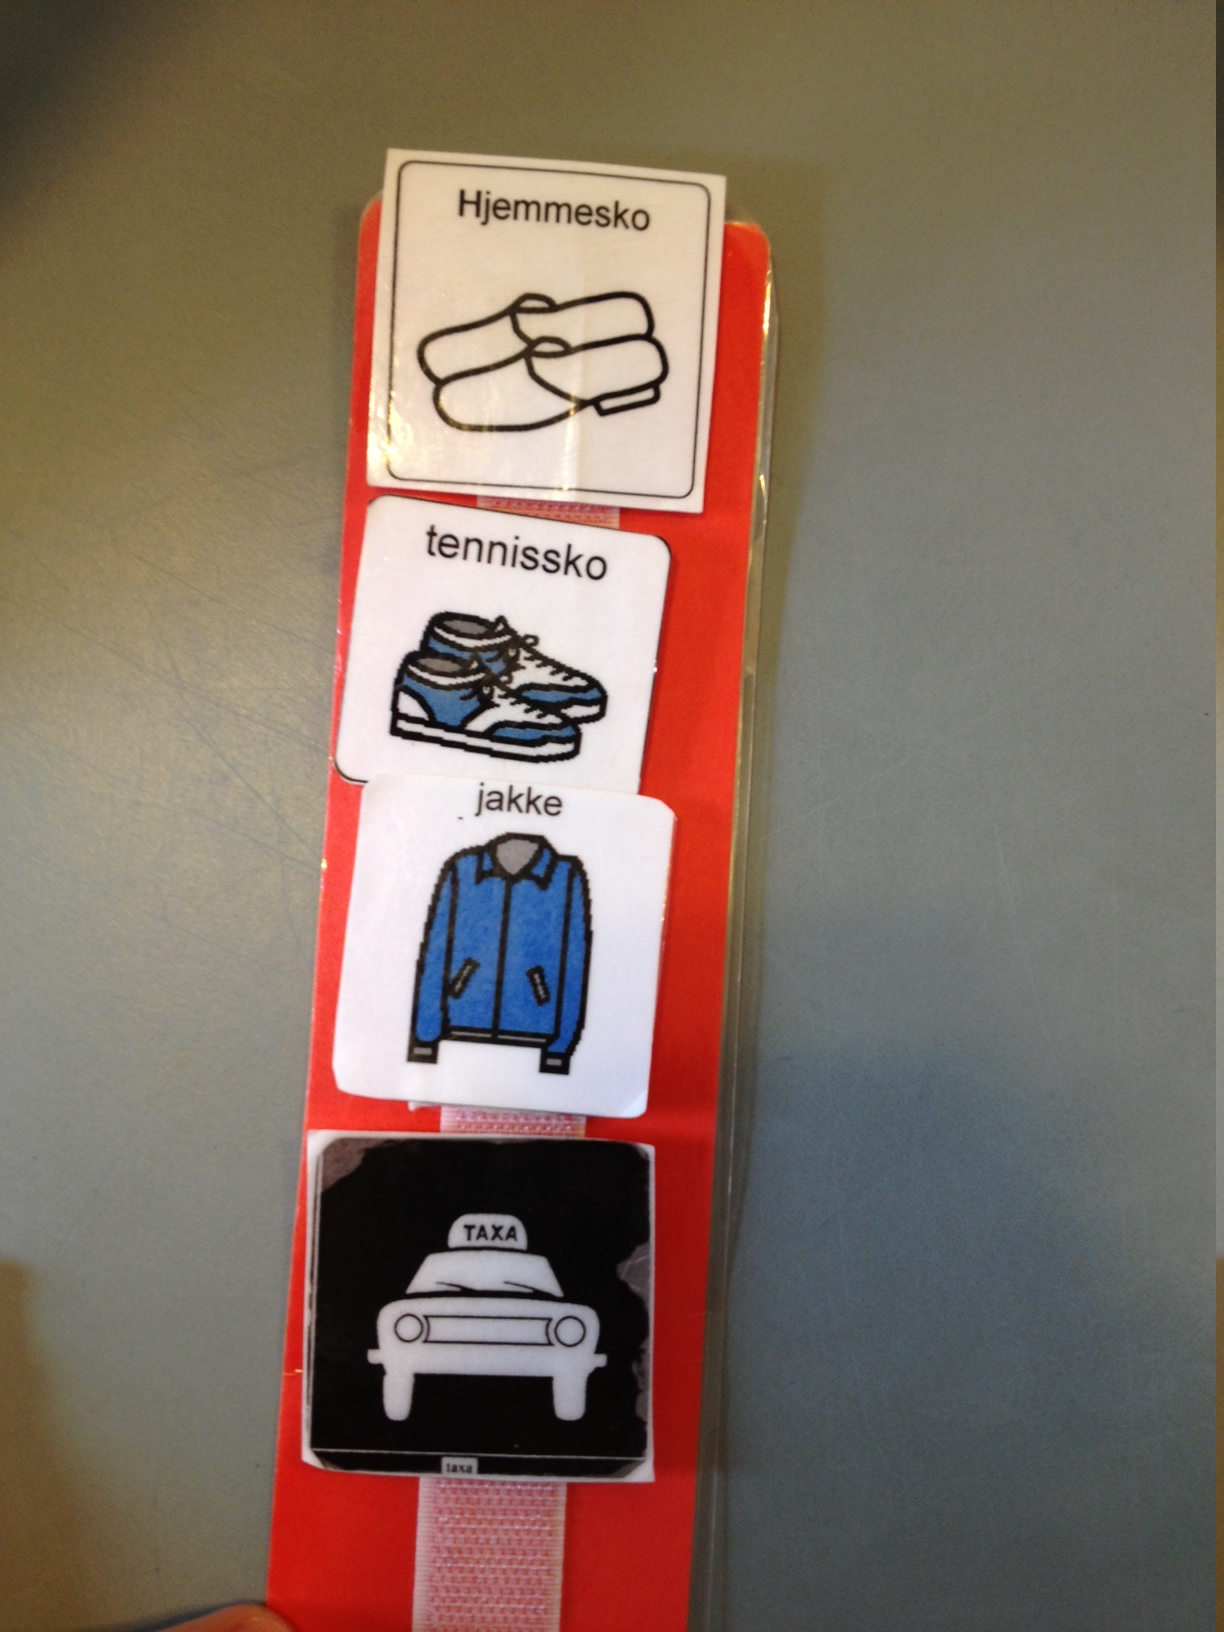
\includegraphics[scale=0.15]{tex/commonReport/img/current_use_picto.jpg}
        \caption{\label{img:pic_current} Pictograms in use 2013}
\end{figure}
During the spring semester of 2013, when this report was written, the use of pictograms is mostly in the form of physical images. The images need to be drawn and/or edited, printed, cut out and then laminated to extend their lifespan. After this process the pictograms are ready for use, generally for one individual, making this repetitive and tedious for the guardians.% \todo{Klim: Bliver dette virkelig kun brugt for et enkelt barn? Kan mapper ikke deles af flere b{\o}rn? Biggi: Nej det kan de ikke, det er blevet sagt af kontakt-person}
When the required amount of pictograms have been created for an individual, they need to be organized and made accessible with the help of some sort of container. This container can be a folder with a pocket for the pictograms and a velcro-like strip for arranging the pictograms. For communication an individual can choose to form sentences by arranging the pictograms accordingly or use a single image to simply express needs and wants. Another purpose of the pictograms is depicted in \autoref{img:pic_current} where instructions are graphically represented for various tasks, in the form of ``do \textbf{A}, followed by \textbf{B} and lastly do \textbf{C}'' for individuals requiring special assistance.

\subsubsection*{Digitizing the Pictogram}
%What's new, what had previous groups implemented, reflect on why it had to be redone.
The \ac{giraf} project focuses on simplifying and digitizing a medium used by individuals with autism and their guardians. This includes digitizing the pictograms, making them available on devices running Android with added functionality. Added functionality includes the option to make the pictograms play a sound, dynamically change the layout of text-labels and editing images. Digitizing the pictogram also makes it possible to share them easily, carry them between devices and make backups of them. Previously, with the same idea in mind, it was attempted to digitize the pictograms. It was considered unsatisfactory (see section below) and therefore the re-implementation in this semester's project.

\subsubsection*{GIRAF Pictogram Design}
%What is the pictogram (basically). What are the ideas behind the current design.
%How is this design better than the previous? How is it used?
The digitized pictogram consists of an image, text-label and a sound. With all elements included, it can be presented as each of the three, two parts combined or all three in union. This viewable container is designed as an extension of the \emph{Android} view class, making it easy for developers to include and present in their applications. The idea is to have users sharing the same pictograms, with the option to customize their contents without affecting the pictogram itself. The previous \ac{giraf} pictogram design lacked documentation, portability and functionality such as text-labels. Therefore a new design was implemented, which hopefully fits the needs of both future \ac{giraf} developers and \ac{giraf} users.
